\chapter{Background}
\label{background}

This chapter provides essential background on Large Reasoning Models (LRMs) and agentic environments, establishing the foundation for understanding the overthinking phenomenon we explore in this thesis.

\begin{figure}[t]
    \centering
    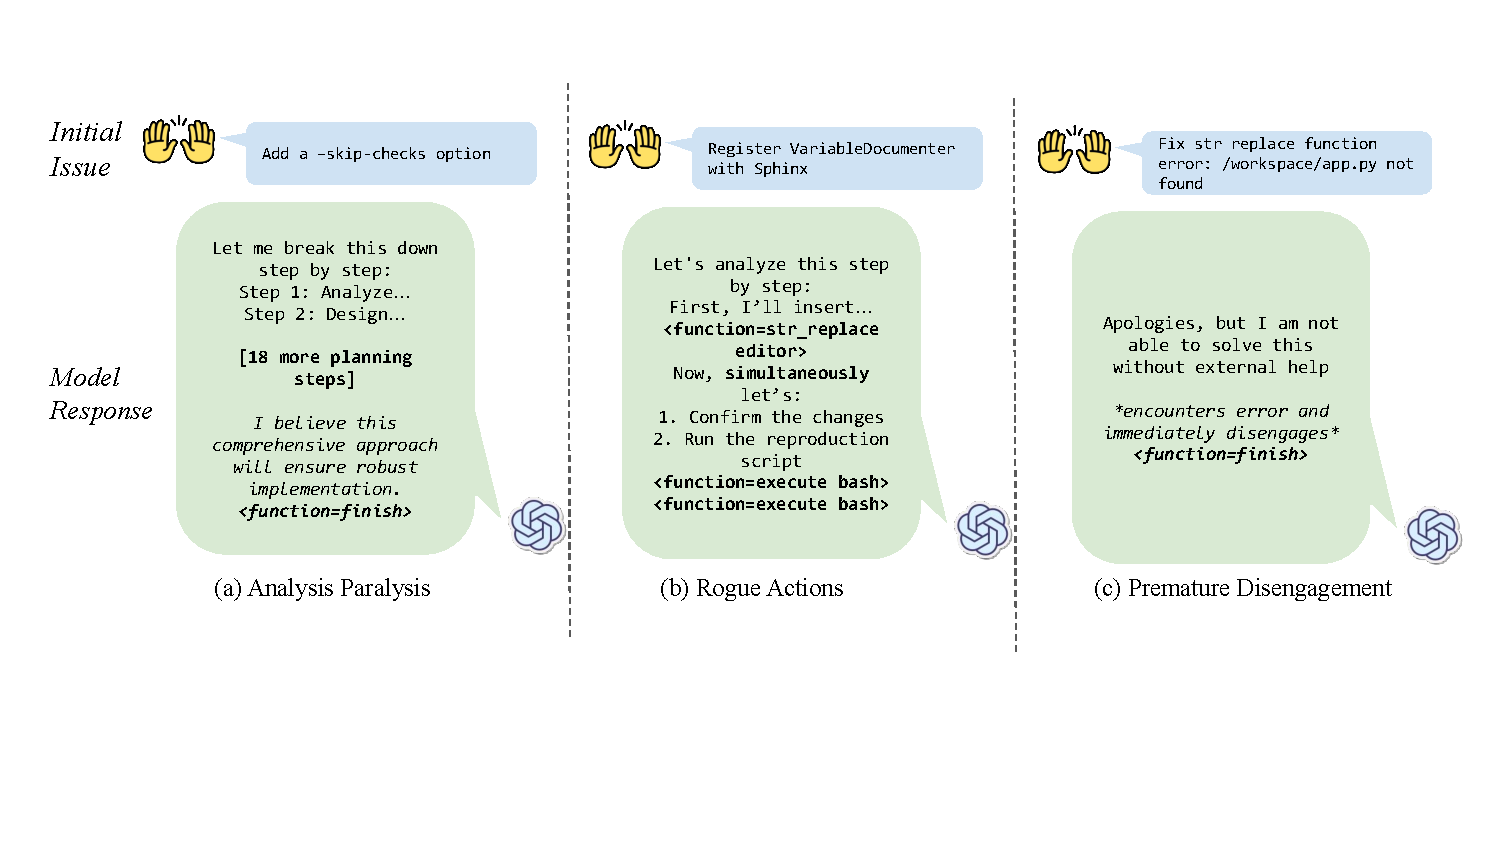
\includegraphics[width=1\linewidth]{manifestations.pdf}
    \caption{Three distinct patterns of overthinking behavior in LRM agent trajectories. (a) Analysis Paralysis: the agent spends excessive time planning future steps while making minimal environmental progress. (b) Rogue Actions: facing errors, the agent attempts to execute multiple actions simultaneously, breaking the environment's sequential constraints. (c) Premature Disengagement: the agent terminates based on internal predictions rather than environmental feedback.}
    \label{fig:manifestations}
\end{figure}

\begin{figure}[t]
    \centering
    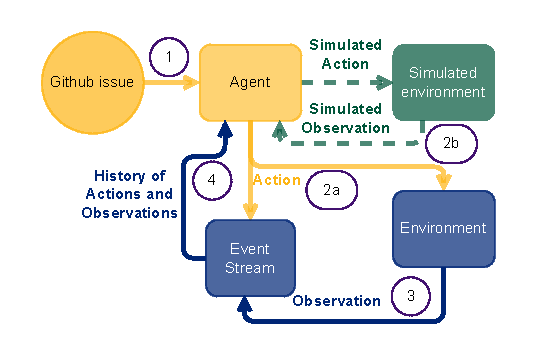
\includegraphics[width=1\linewidth]{figure2.pdf}
    \caption{OpenHands Execution Pipeline. 1) The system initializes by presenting the agent with the primary issue and previous action history. 2) The agent reaches a decision point -- 2a) Direct action formulation and execution, or 2b) Internal simulation of potential actions and outcomes, potentially leading to \textbf{overthinking}. 3) The chosen action is executed, generating environmental feedback which updates the event stream. This cycle continues until task completion.}
    \label{fig:figure3}
\end{figure}

\section{Large Reasoning Models}
\label{sec:lrm}

\subsection{Test-time Computation Scaling}
Test-time computation scaling enhances model performance by allocating additional computational resources during inference. This approach enables LLMs to exceed their baseline training performance, particularly in autonomous agent behaviors and complex reasoning tasks \cite{qu2024recursiveintrospectionteachinglanguage, singh2024humandatascalingselftraining, wei2023chainofthoughtpromptingelicitsreasoning}. Recent studies reveal that training smaller models with reduced computational resources, then augmenting their performance during testing, can yield superior results compared to larger models \cite{snell2024scalingllmtesttimecompute, wu2024inferencescalinglawsempirical}. The O1-mini model exemplifies this approach, surpassing O1-preview's performance on CodeForces \cite{codeforces} and nearly matching the full O1-model's capabilities \cite{openai_learning_to_reason_2024, openai_O1_mini}.

\subsection{Parallel Approaches}
Multiple sampling approaches generate several candidate solutions and select the optimal one through various methods:
\begin{itemize}
    \item Majority voting \cite{huang2022largelanguagemodelsselfimprove}
    \item Best-of-N search \cite{amini2024variationalbestofnalignment}
    \item Sentence-level beam search \cite{graves2012sequencetransductionrecurrentneural}
    \item External verification \cite{lee2024prometheusvisionvisionlanguagemodeljudge, xiong2024llavacriticlearningevaluatemultimodal, brown2024largelanguagemonkeysscaling}
\end{itemize}

While these approaches show promise in certain domains, they face significant limitations in complex software engineering tasks. Majority voting, though effective for standardized problems, struggles with the open-ended nature of SWE-Bench tasks. Best-of-N search, while comprehensive in generating complete solution candidates, introduces substantial complexity in accuracy evaluation. Similarly, sentence-level beam search operates at too fine granularity for effective response quality assessment in software repair contexts \cite{xu2024llavaO1letvisionlanguage}, where the broader solution structure is crucial for success.

\subsection{Sequential Approaches}
LLMs rely on step-by-step reasoning through self-prompting methods, particularly Chain-of-Thought (CoT) \cite{wei2023chainofthoughtpromptingelicitsreasoning}, to implement problem-solving strategies such as:
\begin{itemize}
    \item Systematic Analysis (SA)
    \item Divide and Conquer (DC)
    \item Self-Refinement (SR)
\end{itemize}

Research shows that CoT-based approaches predominantly utilize DC and SR strategies \cite{xu2024llavaO1letvisionlanguage, chu2024navigateenigmaticlabyrinthsurvey}, a pattern also observed in the O1 family of models which builds upon CoT reasoning \cite{openai_reasoning_docs, wu2024comparativestudyreasoningpatterns}. However, CoT's susceptibility to generating incorrect reasoning paths \cite{wei2023chainofthoughtpromptingelicitsreasoning} becomes particularly problematic in repository-level code agents, where models must interact with complex environments and require robust planning and reasoning capabilities \cite{zheng2024makeslargelanguagemodels}.

\section{Agentic Environments}
\label{sec:agentic}

\subsection{OpenHands Framework}
The OpenHands framework provides agents like CodeAct \cite{wang2024executablecodeactionselicit} with tools to interact with the environment. These tools and their usage are provided in-context at the beginning of each prompt, followed by an example of how to interact with the environment using those tools \cite{wang2024openhandsopenplatformai}. 

If the model supports native function calling \cite{openai_function_calling}, these tool descriptions are given through the API and no additional in-context specification is provided. If the model doesn't support native function calling, the successful execution of the action depends on the structured output capabilities of the model. If the tool call is not properly formatted, the environment will return an error and the model will have to adapt it.

\subsection{SWE-Bench}
SWE Bench is a challenging benchmark that requires agents to complete real-world software engineering (SWE) tasks. The agent is given a repository address and an issue description and may need to take many actions to complete the task by producing a final patch \cite{jimenez2024swebenchlanguagemodelsresolve}.

SWE Bench Verified \cite{swebench_verified} is a human-validated subset of SWE Bench \cite{jimenez2024swebenchlanguagemodelsresolve} that more reliably evaluates AI models' ability to solve real-world issues. It contains a validated set of 500 tasks and addresses several limitations of SWE Bench including:
\begin{itemize}
    \item Incorrect grading of correct solutions
    \item Under-specified problem statements
    \item Overly specific unit tests
\end{itemize}

This helps ensure we accurately grade model capabilities \cite{openai_o1_system_card_2024, swebench_verified}. Due to the cost of executing reasoning models \cite{openai_pricing} on multi-stage agentic tasks, we limited our experiments to 200 randomly sampled issues from SWE Bench Verified.

\section{The Reasoning-Action Dilemma}
\label{sec:dilemma}

\subsection{Balancing Internal and External Information}
In agentic environments, models must constantly balance between:
\begin{itemize}
    \item Using their internal knowledge and reasoning capabilities
    \item Gathering new information through environmental interaction
\end{itemize}

This creates a fundamental tension: while internal reasoning can help models plan more effectively, over-reliance on internal simulation can lead to decisions based on incomplete or incorrect assumptions about the environment.

\subsection{The Cost of Overthinking}
Overthinking manifests when models favor extended internal reasoning chains over environmental interaction. This behavior can lead to several issues:
\begin{itemize}
    \item Wasted computational resources on unnecessary reasoning steps
    \item Missed opportunities to gather crucial environmental feedback
    \item Decisions based on outdated or incorrect assumptions
    \item Premature task termination without proper validation
\end{itemize}

Understanding and addressing this balance is crucial for developing more effective AI systems that can operate efficiently in real-world environments.

\section{Evaluation Frameworks}
\label{sec:frameworks}

\subsection{LLM-as-Judge Methodology}
To systematically evaluate overthinking behavior, we employ the LLM-as-judge methodology \cite{zheng2023judgingllmasajudgemtbenchchatbot}, which involves:
\begin{itemize}
    \item Using a separate LLM to evaluate model behavior
    \item Providing clear evaluation criteria and rubrics
    \item Ensuring consistent scoring across different trajectories
    \item Validating automated assessments against human expert judgments
\end{itemize}

\subsection{Statistical Analysis Framework}
Our analysis employs several statistical measures to ensure robust findings:
\begin{itemize}
    \item Coefficient of Determination ($R^2$) to measure correlation strength
    \item P-values to assess statistical significance
    \item Beta coefficients to quantify effect sizes
    \item T-tests to compare different model populations
\end{itemize}

These frameworks provide a rigorous foundation for our analysis of overthinking in LRMs, enabling us to draw reliable conclusions about its impact on model performance.






% \subsection{Industrial Perspectives}

% % \paragraph{Large Enterprise Networks}
% % In order to protect information technology assets, large enterprise networks are partitioned into disjoint segments which group together assets with the same security requirements and policies. These groups are referred to as zones. Zones define the network boundaries and their defense requirements by stating the entities populating the zones, the entry points into the zone as well as how traffic is monitored and filtered at these entry points. Oftentimes, these zones are realized by a (virtualized) separation at layer 2 with firewalls at higher levels governing data transfers between zones.
% Traditionally, enterprises used to consider three security layers for their network 
% environment: intranet, extranet and opennet~\cite{ramasamy2011towards}. The opennet is
% the least trusted network (e.g., the Internet) which is inhospitable region where live 
% threats exist, while the intranet is the most trusted network hosting business-critical 
% systems and sensitive information. Since the intranet has rigorous access controls to 
% protect the information assets from an exposure, enterprises put another security layer 
% (extranet) in between, that only exposes public services to opennet and thus reduces 
% attack surfaces. 
% As enterprises have recently witnessed extreme changes in network environment such as
% diverse demands from customers, partners and employees accessing their network with
% variety of devices, the enterprises employ more sophisticated network security 
% segmentation\cite{obregon2015infrastructure}, called security zones.
% Security zones constitute the logical grouping of one or more subnets that share the
% same security requirements and policies. 
% % Since security zoning is the foundation of 
% % network isolation criteria that must be upheld for secure business environements, 
% % the zone classification of information assets requires 

% Each security zone is identified with different level of trust, and every pair of zones 
% are defined with a namely trusted-untrusted relationship. 
% To realize the unidirectional trust model, firewalls are considered as the most viable
% technologies and widely used in the current practice. However, operating firewalls in 
% large enterprises is often challenging to network operators and security architects. The 
% access control for the security zones might be dynamic, and thus its requires a complex 
% management scheme to accommodate a myriad set of policies. While there are advanced 
% technologies such as virtual firewall~\cite{deng2015vnguard,bakker2016network} and Unified
% Threat Management (UTM)~\cite{qi2007towards}, that are newly designed for enforcement of 
% access control polices in extremely dynamic networks, security zone management and modeling 
% still remains to be evolved~\cite{ramasamy2011towards,gontarczyk2015blueprint}.

% Bridging geographically distant security zones can also be challenging. Oftentimes,
% security zones are created not only for security purpose but also because of geographical
% factors. Given that the security zones in distance should exchange information over
% public network (opennet as aforementioned), there might be a potential risk that the
% communication may expose security-sensitive information during transit. To mitigate
% such a threat, network operators leverage additional security control/mechanisms (e.g.,
% IPSec~\cite{rfc4301} and SSL VPN~\cite{sun2011advantages}) which ensure confidentiality
% and integrity of the transmission over the untrusted network by encrypting the data with
% securely shared cryptographic keys. Nonetheless, the technologies might bring new challenges
% such as management scalability~\cite{felsch2018dangers} and compatibility to the secure 
% isolation~\cite{liu2008collaborative}.

% % \paragraph{Cloud Computing (LaaS, PaaS, SaaS)}
% The cloud computing environment is a good representative example that depicts such practical 
% challenges. Cloud-based service providers operate large multi-tenant data centers which 
% have to scale to customers needs. To achieve this scalability while at the same time staying
% cost efficient cloud providers make heavy use of virtualization techniques. This environment 
% challenges operators with providing secure segmentation between tenants as multiple tenants 
% are using the same physical machines and network. In addition, given that the cloud 
% environments comprise geographically distributed data centers, providing secure communication 
% channels between security zones while upholding a constant view of the security policies
% under the dynamic zone migration is another hill to climb. Now, we derive main challenges 
% we confront in this research with case study.
% % Legal requirements need to be respected. Furthermore, an optimal solution needs to be highly 
% % flexible as the number of assigned resources for a given customer can change frequently.



% % \paragraph{Edge Computing}
% % With the rise of mobile devices and Internet of Things (IoT) new types of data intensive, time
% sensitive applications are emerging. (e.g. VR/AR) However, since these devices are also required to
% be low power they cannot do these heavy computations themselves. Cloud computing can be used to
% offload the work to centralized data centers. However, this causes new challenges. Often, the latency
% between devices and the cloud is too high and therefore not well suited for real-time applications.
% Additionally, a large number of devices means that a centralized infrastructure can get saturated by
% big traffic flows. One widely used solution to this problem is Edge Computing which puts nodes handling
% the computation close to end devices.
